\documentclass{beamer}
\mode<presentation>
{
  \usetheme{Madrid}      % or try Darmstadt, Madrid, Warsaw, ...
  \usecolortheme{beaver} % or try albatross, beaver, crane, ...
  \usefonttheme{serif}  % or try serif, structurebold, ...
  \setbeamertemplate{navigation symbols}{}
  \setbeamertemplate{caption}[numbered]
  \setbeamercolor{theorem}{fg=red}
  \usepackage{amssymb}
  \usepackage{mathtools}

} 

\usepackage[english]{babel}
\usepackage[utf8x]{inputenc}
\usepackage{xcolor}
\usepackage{listings}
\usepackage{wasysym}
\usepackage{tikz}
\usetikzlibrary{tikzmark}
\lstset
{
    language=[LaTeX]TeX,
    breaklines=true,
    basicstyle=\tt\scriptsize,
    %commentstyle=\color{green}
    keywordstyle=\color{magenta},
    stringstyle=\color{black}
    identifierstyle=\color{magenta},
}



\title[]{Introduction to Deep Reinforcement Learning}
\subtitle{
\url{https://github.com/racousin/rl_introduction}}
\author{Raphael Cousin}
\date{January 11, 2024}

\AtBeginSection[]
{
  \begin{frame}<beamer>
    \frametitle{Outline}
    \tableofcontents[currentsection,currentsubsection]
  \end{frame}
}

\begin{document}

\begin{frame}
  \titlepage
\end{frame}
\begin{frame}{Reinforcement Learning Objective}
RL aims to optimize decision-making in environments without a known transition model $P$.

\begin{block}{Objective}
Find the optimal policy $\pi^*$, that maximizes the expected return, $J(\pi)$:
\begin{align*}
\pi^* &= \arg\max_{\pi} J(\pi)\\
J(\pi) &= \mathbb{E}_{\tau\sim\pi}[G(\tau)] = \int_{\tau} \mathbb{P}(\tau|\pi) G(\tau)
\end{align*}
\end{block}

\end{frame}

\begin{frame}{First Glossary of RL}
    \begin{itemize}
        \item Model free/ Model based
        \item Q-learning/Policy Optimization
        \item On-policy/Off-policy
        \item $\epsilon$-Greedy
    \end{itemize}
\end{frame}


\begin{frame}{Overview of RL Algorithms}

        \begin{figure}
        \centering
        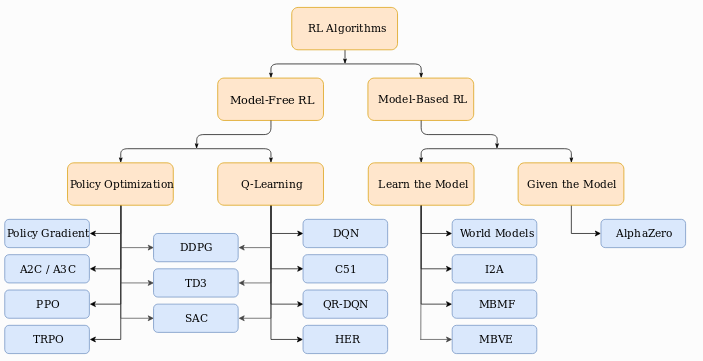
\includegraphics[height=4cm]{tax.png}
    \end{figure}
    \begin{block}{}
    \begin{itemize}
    \item \textbf{Model free:} learn the policy $\pi^*$ directly
    \item  \textbf{Model based:} use an environment model $P^*$ to learn $\pi^*$
\end{itemize}
\end{block}

\end{frame}





\begin{frame}{Key Strategies in Model-Free RL}

\begin{block}{}
    \begin{itemize}
        \item \textbf{Q-learning:} Learn the action-value function \(Q\) to determine the best action given a state:
        \[\pi(s) = \arg\max_{a \in \mathcal{A}} Q_\pi(s, a)\]
        
        \item \textbf{Policy Optimization:} Directly learn the policy \(\pi\) that maximizes the expected return.
    \end{itemize}
\end{block}


\end{frame}





\begin{frame}{Exploration-Exploitation}
Knowledge of the environment comes from interaction. There are trade-offs to be made between using what we know and further exploration.
        \begin{figure}
        \centering
        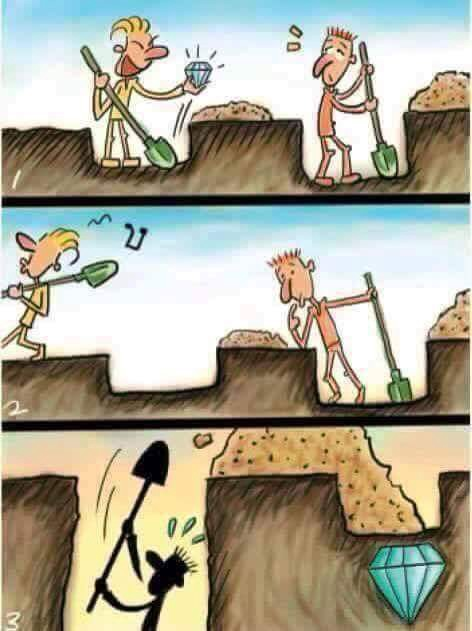
\includegraphics[height=4cm]{images/explore_vs_exploit.jpeg}
    \end{figure}
\end{frame}

\begin{frame}{The \(\epsilon\)-Greedy Strategy}
The \(\epsilon\)-greedy strategy is a simple yet effective method for balancing exploration and exploitation by choosing:

\begin{block}{}
Given a state \(s\), at step \(t\) the policy \(\pi\)  is defined as:
    \begin{itemize}
        \item With probability \(\epsilon\), choose an action at random (exploration).
        \item With probability \(1 - \epsilon\), choose the action with the highest estimated value (exploitation).
    \end{itemize}
\end{block}
\end{frame}

\begin{frame}{Definition}
    \begin{itemize}
    \item{\textbf{On-policy:} Directly learns from and improves the policy it executes.}
    \item{\textbf{Off-policy:} Learns a different policy from the executed one, allowing for learning from observations.}
    \end{itemize}
\end{frame}



\begin{frame}{Second Glossary of RL}
    \begin{itemize}
        \item Monte-Carlo
        \item Temporal difference
        \item SARSA
        \item Q-learning
    \end{itemize}
\end{frame}


\begin{frame}{Monte-Carlo}
\begin{itemize}
\item To evaluate
$V_\pi(s) =  E_{\tau \sim \pi}[{G_t\left| s_t = s\right.}]$
\item Generate an episode with the policy $\pi$ $S_1,A_1,R_2,…,S_T$ to compute $G_t = \sum_{k=0}^{T-t-1} \gamma^k R_{t+k+1}$.
\item The empirical value function is :
 $V_\pi(s) = \frac{\sum_{t=1}^T \mathbb{1}[S_t = s] G_t}{\sum_{t=1}^T \mathbb{1}[S_t = s]}$
 \item As, well, the empirical action-value function is :

 \item $Q_\pi(s, a) = \frac{\sum_{t=1}^T \mathbb{1}[S_t = s, A_t = a] G_t}{\sum_{t=1}^T \mathbb{1}[S_t = s, A_t = a]}$
\end{itemize}
\end{frame}

\begin{frame}{ Monte-Carlo Algorithm}
Initialize Q $Q(s,a) \forall s,a$.
\begin{enumerate}
\item Generate an episode with the policy $\pi$ (extract from $Q$ $\epsilon$-greedy)
\item Update Q using the episode: $q_\pi(s, a) = \frac{\sum_{t=1}^T \big( \mathbb{1}[S_t = s, A_t = a] \sum_{k=0}^{T-t-1} \gamma^k R_{t+k+1} \big)}{\sum_{t=1}^T \mathbb{1}[S_t = s, A_t = a]}$
\item Iterate
\end{enumerate}
\end{frame}

\begin{frame}{Visual Steps in Monte Carlo}

\begin{columns}
    \begin{column}{0.5\textwidth}
        \begin{center}
        % Grid 1: Generate an episode using the policy
        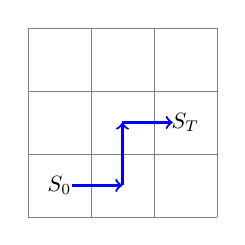
\begin{tikzpicture}[scale=0.8, every node/.style={scale=0.8}]
            \draw[step=1cm,gray,very thin] (0,0) grid (3,3);
            % Path of the episode
            \draw[->, thick, blue] (0.7,0.5) -- (1.5,0.5);
            \draw[->, thick, blue] (1.5,0.5) -- (1.5,1.5);
            \draw[->, thick, blue] (1.5,1.5) -- (2.3,1.5);
            % Start and end states
            \node at (0.5,0.5) {$S_0$};
            \node at (2.5,1.5) {$S_T$};
            % Label
        \end{tikzpicture}
        \end{center}
    \end{column}
    \begin{column}{0.5\textwidth}
        \begin{center}
        % Grid 2: Evaluate Q using the episode
        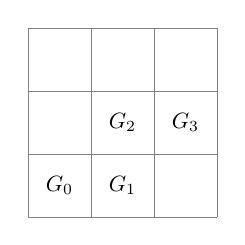
\begin{tikzpicture}[scale=0.8, every node/.style={scale=0.8}]
            \draw[step=1cm,gray,very thin] (0,0) grid (3,3);
            % Highlight the episode path
                        \node at (0.5,0.5) {$G_0$};
                        \node at (1.5,0.5) {$G_1$};
                        \node at (1.5,1.5) {$G_2$};
                        \node at (2.5,1.5) {$G_3$};
            % Label
        \end{tikzpicture}
        \end{center}
    \end{column}
\end{columns}

\bigskip

\begin{columns}
    \begin{column}{0.5\textwidth}
        \begin{center}
        % Grid 4: Iterate the process
        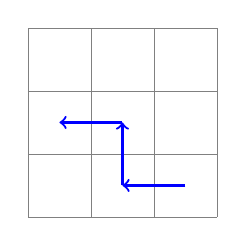
\begin{tikzpicture}[scale=0.8, every node/.style={scale=0.8}]
            \draw[step=1cm,gray,very thin] (0,0) grid (3,3);
            % Highlight the states indicating iteration
            \draw[->, thick, blue] (2.5,0.5) -- (1.5,0.5);
            \draw[->, thick, blue] (1.5,0.5) -- (1.5,1.5);
            \draw[->, thick, blue] (1.5,1.5) -- (0.5,1.5);
            % Label
        \end{tikzpicture}
        \end{center}
    \end{column}
\end{columns}

\end{frame}


\begin{frame}{TD Learning - Key Concepts}
\frametitle{Temporal Difference (TD)}

Monte Carlo and dynamic programming ideas, using bootstrapping for value updates.

\begin{itemize}
    \item \textbf{Bellman equations}:
    \[V(S_t) = \mathbb{E}[R_{t+1} + \gamma V(S_{t+1}) | S_t = s]\]
    \[Q(s, a) = \mathbb{E} [R_{t+1} + \gamma Q(S_{t+1}, A_{t+1}) \mid S_t = s, A_t = a]\]

    \item \textbf{TD Target}: unbiased estimate:
    \begin{itemize}
        \item \(V(S_t)\): \(R_{t+1} + \gamma V(S_{t+1})\)
        \item \(Q(S_t, A_t)\): \(R_{t+1} + \gamma Q(S_{t+1}, A_{t+1})\)
    \end{itemize}
\end{itemize}
\end{frame}
\begin{frame}{Value function estimation with TD Learning}

\begin{block}{TD Error (\(\delta_t\))}
The difference between the TD target and the current value estimate:
\[\delta_t = R_{t+1} + \gamma V(S_{t+1}) - V(S_t)\]
\end{block}

\begin{block}{Update Rule}
Incrementally update the state value with the learning rate (\(\alpha\)):
\[V(S_t) \leftarrow V(S_t) + \alpha \delta_t\]
\end{block}

\end{frame}

\begin{frame}{Action-Value function estimation with TD Learning}

\begin{block}{TD Error (\(\delta_t\))}
The difference between the TD target and the current value estimate:
\[\delta_t = R_{t+1} + \gamma Q(S_{t+1}, A_{t+1}) - Q(S_t, A_t)\]
\end{block}

\begin{block}{Update Rule}
Incrementally update the state value with the learning rate (\(\alpha\)):
\[Q(S_t) \leftarrow Q(S_t) + \alpha \delta_t\]
\end{block}

\end{frame}

 
 \begin{frame}{SARSA Algorithm}
Initialize $Q$ function $Q(s,a) \forall s,a$\\
$S_t=\text{initial state}$, act with $\pi$ (extract from $Q$ $\epsilon$-greedy) to get $A_t,R_{t+1},S_{t+1}$
\begin{enumerate}
\item Act with $\pi$ (extract from $Q$ $\epsilon$-greedy) to get $A_{t+1}, R_{t+2},S_{t+2}$
\item Update Q using the observation step: $Q(S_t, A_t) \leftarrow Q(S_t, A_t) + \alpha (R_{t+1} + \gamma Q(S_{t+1}, A_{t+1}) - Q(S_t, A_t))$\\
\item Iterate
\end{enumerate}
\end{frame}

\begin{frame}{Visual Steps in SARSA}
\begin{center}
% First row of grids
\begin{minipage}{.5\textwidth}
\centering
% Grid 1: Agent chooses an action
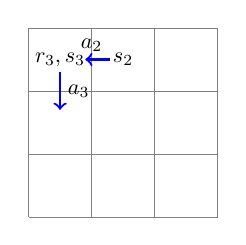
\begin{tikzpicture}[scale=0.8, every node/.style={scale=0.8}]
    \draw[step=1cm,gray,very thin] (0,0) grid (3,3);
    \node at (1.5,2.5) {$s_2$};
    \draw[->, thick, blue] (1.3,2.5) -- (0.9,2.5);
    \node[above] at (1,2.5) {${a_2}$};
    \node at (0.5,2.5) {$r_3, s_3$};
    \draw[->, thick, blue] (0.5,2.3) -- (0.5,1.7);
    \node[right] at (0.5,2) {${a_3}$};
\end{tikzpicture}
\end{minipage}%
\begin{minipage}{.5\textwidth}
\centering
% Grid 2: Update of Q based on s, a, r, s', a'
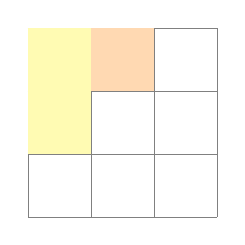
\begin{tikzpicture}[scale=0.8, every node/.style={scale=0.8}]
    \draw[step=1cm,gray,very thin] (0,0) grid (3,3);
    \fill[orange!30] (1,2) rectangle (2,3); % Previous state
    \fill[yellow!30] (0,1) rectangle (1,3); % Current state
\end{tikzpicture}
\end{minipage}

\bigskip % Separation between rows

% Second row of grids
\begin{minipage}{.5\textwidth}
\centering
% Grid 3: Agent chooses next action
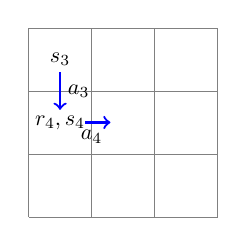
\begin{tikzpicture}[scale=0.8, every node/.style={scale=0.8}]
    \draw[step=1cm,gray,very thin] (0,0) grid (3,3);
    \node at (0.5,2.5) {$s_3$};
    \draw[->, thick, blue] (0.5,2.3) -- (0.5,1.7);
    \node[right] at (0.5,2) {${a_3}$};
    \node at (0.5,1.5) {$r_4,s_4$};
    \draw[->, thick, blue] (0.9,1.5) -- (1.3,1.5);
    \node[below] at (1,1.5) {${a_4}$};
\end{tikzpicture}
\end{minipage}%
\begin{minipage}{.5\textwidth}
\centering
% Grid 4: Final update of Q
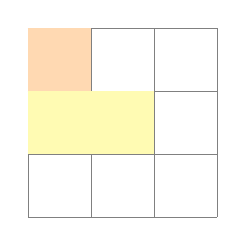
\begin{tikzpicture}[scale=0.8, every node/.style={scale=0.8}]
    \draw[step=1cm,gray,very thin] (0,0) grid (3,3);
    \fill[orange!30] (0,2) rectangle (1,3); % Previous state
    \fill[yellow!30] (0,1) rectangle (2,2); % Current state
\end{tikzpicture}
\end{minipage}
\end{center}
\end{frame}








\begin{frame}{Q-learning}
\begin{itemize}
 \item Remember $Q_{\pi^*}(S_t,A_t) = \mathbb{E} [R_{t+1} + \gamma \max_{a'} Q_*(S_{t+1}, a') \vert S_t = s, A_t = a]$
 \item So $R_{t+1} + \gamma \max_{a'} Q(S_{t+1}, a')$ is an unbiased estimate for $Q(S_t, A_t)$
  \item $R_{t+1} + \gamma \max_{a'} Q(S_{t+1}, a')$ is called the Q target.
   \item $\alpha$ improvement:\\ $Q(S_t, A_t) \leftarrow Q(S_t, A_t) + \alpha (R_{t+1} + \gamma \max_{a \in \mathcal{A}} Q(S_{t+1}, a) - Q(S_t, A_t))$
\end{itemize}

\end{frame}
 
 \begin{frame}{Q-learning Algorithm}
Initialize $Q$ function $Q(s,a) \forall s,a$\\
$S_t=\text{initial state}$
\begin{enumerate}
\item Act with $\pi$ (extract from $Q$ $\epsilon$-greedy) to get $A_{t}, R_{t+1},S_{t+1}$
\item Update $Q$ using the observation step: $Q(S_t, A_t) \leftarrow Q(S_t, A_t) + \alpha (R_{t+1} + \gamma \max Q(S_{t+1}, a) - Q(S_t, A_t))$\\
\item Iterate
\end{enumerate}
\end{frame}

\begin{frame}{Visual Steps in Q-Learning}
\begin{center}
% First row of grids
\begin{minipage}{.5\textwidth}
\centering
% Grid 1: Agent chooses an action
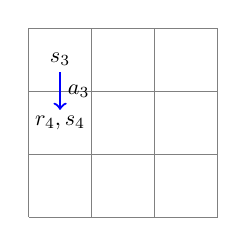
\begin{tikzpicture}[scale=0.8, every node/.style={scale=0.8}]
    \draw[step=1cm,gray,very thin] (0,0) grid (3,3);
    \node at (0.5,2.5) {$s_3$};
    \draw[->, thick, blue] (0.5,2.3) -- (0.5,1.7);
    \node[right] at (0.5,2) {${a_3}$};
    \node at (0.5,1.5) {$r_4, s_4$};
\end{tikzpicture}
\end{minipage}%
\begin{minipage}{.5\textwidth}
\centering
% Grid 2: Update of Q based on s, a, r, s', a'
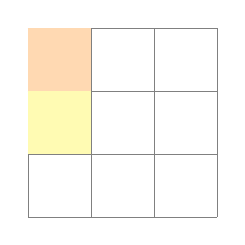
\begin{tikzpicture}[scale=0.8, every node/.style={scale=0.8}]
    \draw[step=1cm,gray,very thin] (0,0) grid (3,3);
    \fill[orange!30] (0,2) rectangle (1,3); % Previous state
    \fill[yellow!30] (0,1) rectangle (1,2); % Current state
\end{tikzpicture}
\end{minipage}

\bigskip % Separation between rows

% Second row of grids
\begin{minipage}{.5\textwidth}
\centering
% Grid 3: Agent chooses next action
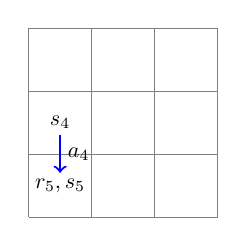
\begin{tikzpicture}[scale=0.8, every node/.style={scale=0.8}]
    \draw[step=1cm,gray,very thin] (0,0) grid (3,3);
    \node at (0.5,1.5) {$s_4$};
    \draw[->, thick, blue] (0.5,1.3) -- (0.5,0.7);
    \node[right] at (0.5,1) {${a_4}$};
        \node at (0.5,0.5) {$r_5, s_5$};
\end{tikzpicture}
\end{minipage}%
\begin{minipage}{.5\textwidth}
\centering
% Grid 4: Final update of Q
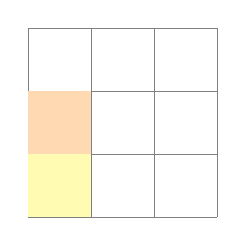
\begin{tikzpicture}[scale=0.8, every node/.style={scale=0.8}]
    \draw[step=1cm,gray,very thin] (0,0) grid (3,3);
    \fill[orange!30] (0,1) rectangle (1,2); % Previous state
    \fill[yellow!30] (0,0) rectangle (1,1); % Current state
\end{tikzpicture}
\end{minipage}
\end{center}
\end{frame}

\begin{frame}[plain,c]
\begin{center}
\Huge Coding session

Temporal Difference
\end{center}
\end{frame}

\begin{frame}{Third Glossary of RL}
    \begin{itemize}
        \item Reinforce/VPG
        \item Deep Q-learning
        \item Actor-Critic
    \end{itemize}
\end{frame}


\begin{frame}{Limitations of Traditional Q Learning}
Q Learning faces challenges when scaling to complex problems:
\begin{itemize}
    \item High-dimensional state spaces lead to slow convergence.
    \item Inapplicable to environments with continuous action spaces.
\end{itemize}
\end{frame}


\begin{frame}{Deep Q Learning Overview}
Deep Q Learning extends Q Learning by using neural networks:
\begin{itemize}
    \item Parametrize \(Q\) function with \(\theta\), \(Q_\theta : S \times A \rightarrow \mathbb{R}\).
    \item Objective: Find \(\theta^*\) that approximates the optimal \(Q\) function.
    \item Define Q target as: \(y = R_{t+1} + \gamma \max_{a'} Q_\theta(S_{t+1}, a')\).
    \item Minimize loss (e.g., MSE): \(L(\theta) = \mathbb{E}_{s,a \sim Q} [(y - Q(s,a,\theta))^2]\).
\end{itemize}
\end{frame}
\begin{frame}{Executing the Deep Q Learning Algorithm}
Steps to implement Deep Q Learning:
\begin{enumerate}
    \item For current state \(S_t\), compute \(Q_\theta(S_t, a)\) for all actions.
    \item Take action \(A_t\) with highest \(Q\) value, observe reward and next state.
    \item Compute target \(y\) for \(S_{t+1}\) and minimize loss \(L(\theta)\).
    \item Iterate to refine \(\theta\) towards optimal.
\end{enumerate}
\end{frame}
\begin{frame}{Improving Deep Q Learning Stability}
Key techniques for enhancing DQL:
\begin{itemize}
    \item \textbf{Experience Replay}: Store transitions \((S_t, A_t, R_{t+1}, S_{t+1})\) and sample randomly to break correlation in sequences.
    \item \textbf{Target Network}: Use a separate, slowly updated network to stabilize targets.
    \item \textbf{Additional Improvements}: Epsilon decay for exploration, reward clipping, Double Q Learning to reduce overestimation.
\end{itemize}
\end{frame}


\begin{frame}[plain,c]
\begin{center}
\Huge Coding session

Deep Q - learning
\end{center}
\end{frame}

\begin{frame}{Policy Optimization}
    \begin{itemize}
 \item Parametrization of policy, $\pi_{\theta}$.
 \item We aim to maximize the expected return $J(\pi_{\theta}) = E_{\tau \sim \pi_{\theta}}[{G(\tau)}]$.\\

 \item Gradient ascent:\\
$\theta_{k+1} = \theta_k + \alpha \left. \nabla_{\theta} J(\pi_{\theta}) \right|_{\theta_k}$.

 \item We can proof  that:\\
$\nabla_{\theta} J(\pi_{\theta}) = E_{\tau \sim \pi_{\theta}}[{\sum_{t=0}^{T} \nabla_{\theta} \log \pi_{\theta}(a_t |s_t) G(\tau)}]$ 


\url{https://lilianweng.github.io/lil-log/2018/04/08/policy-gradient-algorithms.html}

\end{itemize}
\end{frame}
\begin{frame}{Reinforce/VPG algorithm}
Initialize policy $\pi_{\theta}$
\begin{enumerate}
    \item Generate episodes $\mathcal{D} = \{\tau_i\}_{i=1,...,N}$ with the policy $\pi_\theta$
     \item Compute gradient approximation $\hat{\nabla} = \frac{1}{|\mathcal{D}|} \sum_{\tau \in \mathcal{D}} \sum_{t=0}^{T} \nabla_{\theta} \log \pi_{\theta}(a_t |s_t) G_t$
    \item Update policy (apply gradient ascent) $\theta \leftarrow \theta + \alpha \hat{\nabla}$ 
    \item Iterate
\end{enumerate}
\end{frame}


\begin{frame}{Introduction to Actor-Critic Models}
Actor-Critic models combine the benefits of policy-based and value-based approaches:
\begin{itemize}
    \item The \textbf{Actor} updates the policy distribution in the direction suggested by the \textbf{Critic}.
    \item The \textbf{Critic} estimates the value function (\(V\) or \(Q\)) to critique the actions taken by the Actor.
    \item This interaction enhances learning by using the Critic’s value function to reduce the variance in policy gradient estimates.
\end{itemize}
\end{frame}
\begin{frame}{Policy Gradient in Actor-Critic}
The policy gradient in Actor-Critic models can be written as:
\[\nabla_{\theta} J(\pi_{\theta}) = E_{\tau \sim \pi_{\theta}}\left[\sum_{t=0}^{T} \nabla_{\theta} \log \pi_{\theta}(a_t |s_t) \Phi_t\right]\]

Where \(\Phi_t\) represents:
\begin{itemize}
    \item Total return \(G_t\).
    \item Advantage function: \(R_{t+1} - V(s_t)\) or \(R_{t+1} - Q(s_t, a_t)\).
\end{itemize}
Using \(\Phi_t\) improves policy updates by evaluating actions more effectively.
\end{frame}
\begin{frame}{Actor-Critic Algorithm Steps}
Implementing the Actor-Critic algorithm involves:
\begin{enumerate}
    \item Initializing parameters for both the Actor (\(\theta\)) and the Critic (\(\phi\)).
    \item For each episode:
        \begin{enumerate}
            \item Generate an action \(A_t\) using the current policy \(\pi_{\theta_t}\).
            \item Update the Actor by applying gradient ascent using the Critic's feedback.
            \item Update the Critic by minimizing the difference between estimated and actual returns.
        \end{enumerate}
    \item Repeat the process to refine both Actor and Critic.
\end{enumerate}
\end{frame}


\begin{frame}{References}
\textbf{Course:}\\
\url{http://incompleteideas.net/book/the-book-2nd.html}\\
\url{https://lilianweng.github.io/lil-log/2018/02/19/a-long-peek-into-reinforcement-learning.html}\\
\url{http://rail.eecs.berkeley.edu/deeprlcourse-fa17/f17docs/}\\
\url{https://github.com/kengz/awesome-deep-rl}\\
\textbf{Framework:}\\
\url{https://spinningup.openai.com/en/latest/}\\
\url{https://gym.openai.com/envs/#atari}\\
\url{https://github.com/deepmind/bsuite}
\end{frame}
\end{document}
